\documentclass[titlepage,a4paper,oneside]{article}
\usepackage[utf8]{inputenc}
\usepackage{amsmath}
\usepackage{mathabx}
\usepackage{graphicx}
\usepackage{minted}
\usepackage{booktabs}
\usepackage[english,spanish,es-noindentfirst,es-nosectiondot,es-nolists,
es-noshorthands,es-lcroman,es-tabla]{babel}
\usepackage{lmodern}             % Use Latin Modern fonts
\usepackage[T1]{fontenc}         % Better output when a diacritic/accent is used
\usepackage[utf8]{inputenc}      % Allows to input accented characters
\usepackage{textcomp}            % Avoid conflicts with siunitx and microtype
\usepackage{microtype}           % Improves justification and typography
\usepackage[svgnames]{xcolor}    % Svgnames option loads navy (blue) colour
\usepackage[hidelinks,urlcolor=blue]{hyperref}
\hypersetup{colorlinks=true, allcolors=Navy, pdfstartview={XYZ null null 1}}
\newtheorem{lemma}{Lema}
\usepackage[width=14cm,left=3.5cm,marginparwidth=3cm,marginparsep=0.35cm,
height=21cm,top=3.7cm,headsep=1cm, headheight=1.6cm,footskip=1.2cm]{geometry}
\usepackage{csquotes}
\usepackage{biblatex}
\addbibresource{informe.bib}

\begin{document}

\begin{titlepage}
\title{
	75.74 \-- Distribuidos I \-- TP1\\
    \large Facultad de Ingeniería\\
	Universidad de Buenos Aires
}
\author{
	Mermet, Ignacio Javier\\
	\texttt{98153}
}
\date{Abril 2022}

\maketitle

\end{titlepage}

\tableofcontents

\newpage

\section{Sobre la entrega}
El código de la entrega se puede encontrar en \href{https://github.com/CrossNox/7574-TP1}{GitHub}.

\section{Estructura del proyecto}
El proyecto fue desarrollado en \texttt{python}\cite{Python} y empaquetado con \texttt{poetry}\cite{PythonPoetry}. Tiene dos CLIs asociadas:

\begin{itemize}
	\item \texttt{metrics\_server}: el servidor de métricas
	\item \texttt{metrics\_client}: cliente para enviar, consultar y monitorear métricas
\end{itemize}

En la carpeta \texttt{docker} se encuentran disponibles los \texttt{Dockerfile} asociados tanto al servidor como al cliente.

\section{Instalación y ejecución}
Referirse al archivo \texttt{README.md} provisto en el repositorio para ver las instrucciones de instalación.

\subsubsection{Ejecución del server}

A continuación se muestra la ayuda de la CLI asociada al servidor.

\begin{figure}[H]
\begin{minted}[
	mathescape,
	linenos,
    numbersep=5pt,
	gobble=0,
	frame=lines,
	framesep=2mm]{bash}
$ poetry run metrics_server --help
Usage: metrics_server [OPTIONS]

Options:
  --host TEXT                     Host to bind server to  [default: 0.0.0.0]
  --port INTEGER                  Port to bind the server to  [default: 5678]
  --workers INTEGER               Amount of processes handling metrics
                                  [default: 16]
  --backlog INTEGER               How many unaccepted connections the system
                                  allows before refusing new ones  [default:
                                  8]
  --writers INTEGER               Amount of processes writing metrics to disk
                                  [default: 16]
  --queriers INTEGER              Amount of processes handling queries
                                  [default: 4]
  --notifiers INTEGER             Amount of processes reviewing active
                                  notifications  [default: 4]
  --data-path PATH                Path to save data to  [default: /tmp]
  --notifications-log-path PATH   Path to write notification messages to
                                  [default:
                                  /tmp/metrics_server_notifications.log]
  --notifications-cfg TEXT        Path to notifications configuration ini file
                                  [default: /home/nox/repos/fiuba/7574-Distrib
                                  uidosI/7574-TP1/notifications.ini]
  -v, --verbose                   Level of verbosity. Can be passed more than
                                  once for more levels of logging.  [default:
                                  0]
  --pretty                        Whether to pretty print the logs with colors
\end{minted}
\caption{Mensaje de ayuda de la CLI del servidor.}
\end{figure}

La configuración de la ejecución se hace a través de un archivo \texttt{.ini} en el root del proyecto o bien por variables de entorno. La sección \ref{configuracion} provee mayor detalle.

\subsection{Cliente de ejemplo}
A continuación se muestra la ayuda de la CLI asociada al cliente provisto.

\begin{figure}[H]
\begin{minted}[
	mathescape,
	linenos,
    numbersep=5pt,
	gobble=0,
	frame=lines,
	framesep=2mm]{bash}
$ poetry run metrics_client --help
Usage: metrics_client [OPTIONS] COMMAND [ARGS]...

Options:
  --host TEXT                     Host address of the server  [default:
                                  0.0.0.0]
  --port INTEGER                  Port of the server  [default: 5678]
  --retries INTEGER               Retries to connect to the server  [default:
                                  5]
  -v, --verbose                   Level of verbosity. Can be passed more than
                                  once for more levels of logging.  [default:
                                  0]
  --pretty                        Whether to pretty print the logs with colors

Commands:
  monitor  Monitor triggered notifications.
  query    Send a query to the server and print the result.
  ramp     Send a burst of metrics to a server.
  send     Send a single metric to a server.
\end{minted}
\caption{Mensaje de ayuda de la CLI del cliente.}
\end{figure}

Vemos que hay cuatro subcomandos disponibles: dos modos de envío de métricas, consultas y monitoreo de notificaciones.

Para ver el mensaje de ayuda de alguno de los subcomandos, se puede hacer con \texttt{poetry run metrics\_client <subcomando> \--\--help}.

\subsection{Configuración} \label{configuracion}
En el root del proyecto se encuentra un archivo \texttt{sample\_settings.ini}, donde se ven los posible valores a configurar:

\begin{figure}[H]
\begin{minted}[
	mathescape,
	linenos,
    numbersep=5pt,
	gobble=0,
	frame=lines,
	framesep=2mm]{ini}
[server]
host=0.0.0.0
port=5678
workers=16
backlog=8
writers=16
queriers=4
notifiers=4
data_path=/tmp
notifications_log_path=/tmp/metrics_server_notifications.log
notifications_cfg=/var/notifications.ini
\end{minted}
\caption{Archivo de configuración de ejemplo.}
\end{figure}

El proyecto, sin embargo, espera un archivo llamado \texttt{settings.ini}. Por motivos obvios de seguridad, este archivo es ignorado en el sistema de versionado.

Puede copiar el archivo de prueba provisto, renombrarlo y modificar los valores según necesidad.

Cada posible configuración se puede sobreescribir con variables de entorno con la nomenclatura \texttt{<Sección>\_<Clave>}. Por ejemplo \texttt{SERVER\_HOST}.

\section{Arquitectura general}
\subsection{Diagrama de robustez} \label{robustez}
\begin{figure}[H]
\centering
\includegraphics[width=\textwidth]{images/diagrama_robustez.png}
\caption{Diagrama de robustez}
\end{figure}

\subsubsection{Server loop}
El server loop acepta las conexiones entrantes y las mete en \texttt{Connections queue} para ser despachadas al \textit{handler} adecuado.

\subsubsection{Connection dispatcher}
Es proceso se encarga tomar las conexiones entrantes en \texttt{Connections queue}, revisar el \textit{intention} declarado por la conexión y luego despacharla a la queue correspondiente a ese \textit{intention}.

\subsubsection{Metrics handlers}
Estos procesos se encargan de tomar conexiones desde \texttt{Metrics conns queue} y recibir todas las métricas enviadas desde ese cliente. Cada métrica recibida se mete en una queue de entre \texttt{Metrics queues} según \eqref{crcindex}.

\subsubsection{Metrics writers}
Cada proceso de este tipo toma métricas de una queue en particular y se encarga de escribirlas a archivos, particionando por \texttt{metric\_id} y por \texttt{timestamp}.

\subsubsection{Queries handlers}
Estos procesos se encargan de tomar una conexión desde \texttt{Queries conns queue}, recibir la query enviada desde la conexión, leer los archivos correspondientes a la métrica y período pedidos, y sobre ellos calcular las agregaciones requeridas. Luego envían este valor por la conexión establecida.

\subsubsection{Notifications workers}
Al levantar el servidor, se lee la configuración de notificaciones y cada elemento se carga en la queue \texttt{Notifications queue}. Estos procesos se encargan de tomar una notificación desde la queue y revisar si es momento de ejecutarla, colocándola de nuevo en la queue si no lo fuera. Si lo fuera, se realiza la query correspondiente. Si la query arrojara un valor que supere el umbral definido, se coloca en la queue \texttt{Notifications messages queue} el mensaje correspondiente.

\subsubsection{Notifications messages handler}
Este proceso se encarga de distribuir a donde corresponde los mensajes de notificaciones. Por un lado escribe a un archivo los mensajes.

Por otro lado, toma conexiones desde \texttt{Notifications conns queue} y las agrega a una lista interna de conexiones. Cada nuevo mensaje de notificación es enviado a estos clientes también.

\subsection{Diagrama de clases}
\begin{figure}[H]
\centering
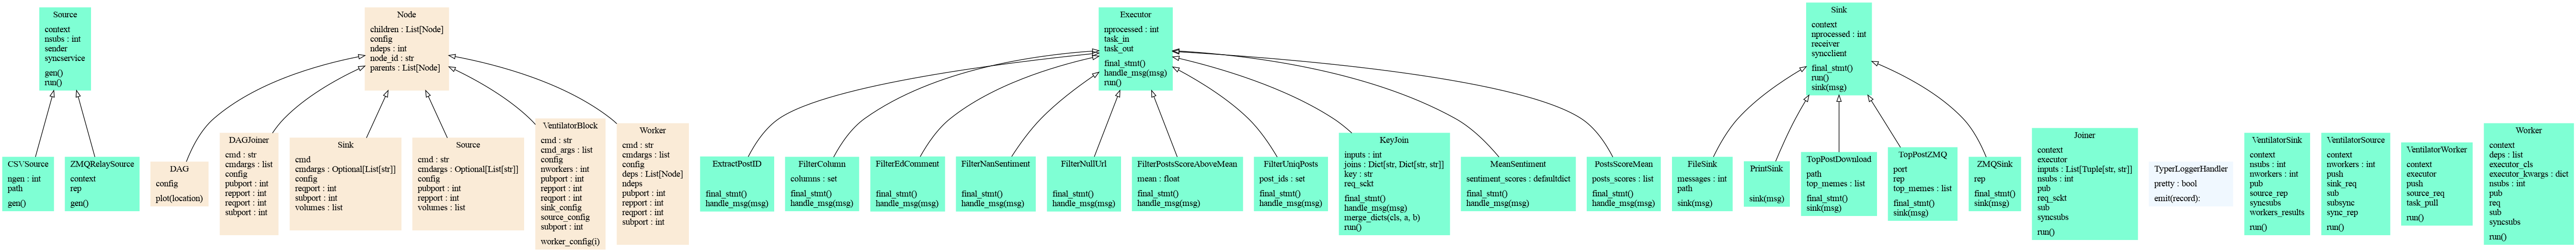
\includegraphics[width=\textwidth]{images/classes.png}
\caption{Diagrama de clases - generado automáticamente con \texttt{pyreverse}}
\end{figure}

\subsection{Diagrama de paquetes}
\begin{figure}[H]
\centering
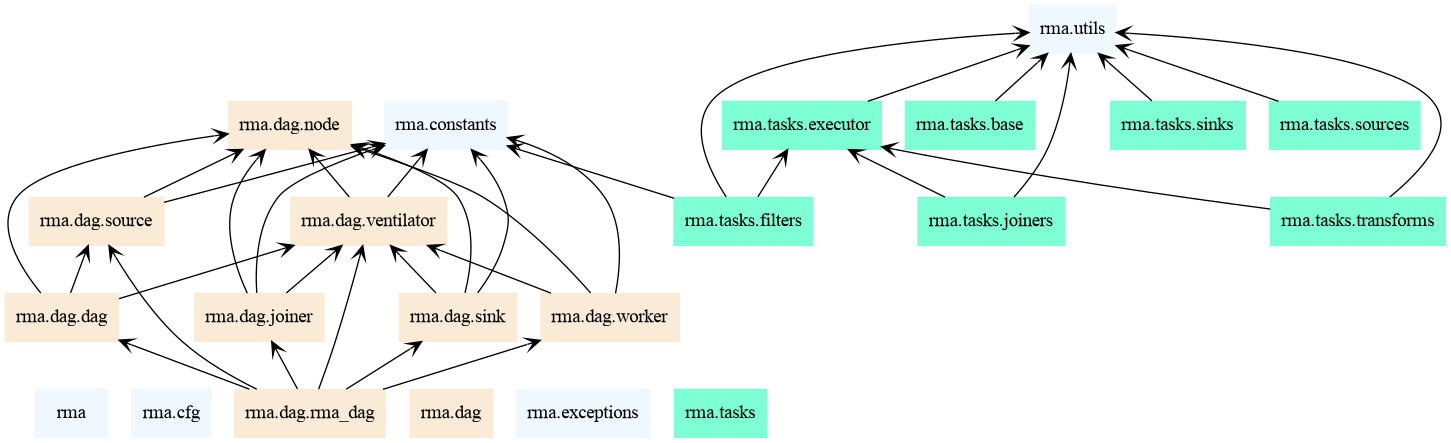
\includegraphics[width=\textwidth]{images/packages.png}
\caption{Diagrama de paquetes - generado automáticamente con \texttt{pyreverse}}
\end{figure}

\subsection{Notas sobre escalabilidad}
El sistema permite configurar la cantidad de procesos que procesan métricas, queries y notificaciones. Si fuéramos a recibir muchas conexiones, tener un solo despachador de conexiones podría ser un cuello de botella.

Por otro lado, se puede argumentar que tener un solo manejador de mensajes de notificaciones no sería un cuello de botella: no debieran saltar demasiadas alarmas al mismo tiempo, asumiendo que los sistemas que reportan métricas funcionan razonablemente bien y que las notificaciones están configuradas con valores sensatos.

El uso de colas para manejar la concurrencia hace que varios de los componentes del sistema escalen a un escenario multicomputing. Sin embargo, hay que tener algunas consideraciones.

Asumamos que la cantidad de queues de métricas es constante. Sea $M_i$ el identificador de la i-ésima métrica que se ha recibido. $M_i$ se asigna a la queue $Q_j$ donde

\begin{equation}\label{crcindex}
	j = \text{crc}(M_i) \mod \mid \text{Queues de métricas} \mid
\end{equation}

El proceso $W_j$ toma métricas de la queue $Q_j$ y las escribe a disco, particionadas por identificador de la métrica y por minuto del timestamp de la métrica recibida. Notar que $M_i$ \textbf{siempre} es escrita por $W_j$.

Un proceso $Y_j$ que resuelva consultas sobre una métrica $M_i$ debe o bien ser ejecutado en la misma máquina que el proceso $W_j$ o tener acceso al filesystem de $W_j$.

El segundo caso no es trivial de resolver. Tecnologías como HDFS\cite{HDFS} involucran una gran cantidad de ingeniería que, se entiende, supera los objetivos del presente trabajo práctico.

Para poder resolver el primer escenario se puede replicar lo que se usa para escribir las métricas: mandar cada query $Q_x$ sobre la métrica $M_i$ a una queue. El proceso $Y_j$ vive en la misma máquina que $W_j$, toma la query de la queue y la ejecuta, teniendo acceso a los archivos de $M_i$.

Si la cantidad de queues de métricas/cantidad de procesos que escriben métricas a archivos cambiase, se deberían reshufflear los archivos de todas las métricas a la máquina correspondiente. Este proceso podría demorar levantar el server para poder recibir métricas y responder queries.

\section{Protocolo de comunicación}
La comunicación cliente-servidor utiliza un protocolo binario. La comunicación se inicia enviando un paquete \texttt{Intention}\cite{IntentionPackage} que indica que tipo de operación se desea ejecutar:
\begin{itemize}
	\item Enviar métrica
	\item Consultar métrica
	\item Monitorear notificaciones
\end{itemize}

Luego el protocolo de comunicación continúa de acuerdo a cada caso particular. Los tamaños de los paquetes corresponden al struct de \texttt{C} subyacente:

\begin{table}[H]
\centering
\begin{tabular}{c|c|c}
\textit{Paquete}     & \textit{String de formato} & \textit{Tamaño del paquete}  \\
\hline
IntentionPackage     & !i                         & 4                            \\
Metric               & !28pL                      & 32                           \\
Query                & !28p12pddd                 & 64                           \\
QueryPartialResponse & !Hf?                       & 7                            \\
ReceivedMetric       & !28pdf                     & 40                           \\
NotificationResponse & !d128p?H                   & 139                          \\
MetricResponse       & !H                         & 2
\end{tabular}
\end{table}

Notar que se espera tamaño \textit{standard} sin alineación, con bytes en orden de red (big-endian).

Para poder desarrollar un ecosistema de aplicaciones que puedan utilizar este protocolo, se debería desarrollar una guía que explique en profundidad que representa cada campo del string de formato de cada paquete.

\subsection{Envío de métrica}
\begin{figure}[H]
\centering
\includegraphics[width=\textwidth]{images/envio_metricas.png}
\caption{Diagrama de secuencia \-- envío de métricas}
\end{figure}

\subsection{Consulta de métrica}
\begin{figure}[H]
\centering
\includegraphics[width=\textwidth]{images/query.png}
\caption{Diagrama de secuencia \-- envío de métricas}
\end{figure}

\subsection{Monitoreo de notificaciones}
\begin{figure}[H]
\centering
\includegraphics[width=\textwidth]{images/notificaciones.png}
\caption{Diagrama de secuencia \-- monitoreo de notificaciones}
\end{figure}

\section{Resolución de concurrencia}
La concurrencia entre distintos procesos se resuelve, en su totalidad, con el uso de queues. De este modo podemos escalar fácilmente la cantidad de procesos de cada tipo, tomando su entrada desde la queue correspondiente y, de ser necesario, dejando su resultado en otra queue.

Para entender como se relacionan los procesos y las queues, referirse a \ref{robustez}.

\subsection{Concurrencia entre lectura y escritura de archivos}
Cada archivo de una métrica $M_i$ es escrito solo por un proceso $W_j$, por tanto no hay concurrencia \texttt{WW} a resolver. La concurrencia \texttt{RW} puede darse en el caso que un proceso esté leyendo el archivo para resolver una query mientras otro sigue escribiendo métricas al mismo.

Sin embargo, al leer, lo que puede pasar es que haya líneas incompletas. Originalmente el CSV se escribía con los campos \texttt{timestamp}, \texttt{metric\_id}, \texttt{value}. Podemos pensar varios escenarios:
\begin{itemize}
	\item El caso feliz: Tenemos todos los campos y el \texttt{\slash n} que termina la línea
	\item Un caso poco feliz, pero poco problemático: tenemos una coma, pero no el valor que sigue
	\item Un caso sutilmente problemático: que el campo \texttt{value} esté truncado!
\end{itemize}

El segundo caso se puede resolver sencillamente ignorando las lineas que no tengan todos los campos. El tercer caso no podemos resolverlo con el esquema de datos planteado. Por tanto se agrega una cuarta columna \texttt{check}, que es una función de \texttt{timestamp}. Para poder escribir rápidamente las líneas, necesitamos que sea una función rápida, un hash quizás sea demasiado lento. Por tanto se prefirió usar la función $\mod 10$. Luego al momento de leer, descartamos las lineas donde $\text{timestamp} \mod 10 \neq \text{check}$.

Por otro lado, se ignoran todas las lineas de momentos anteriores al momento donde se empieza a ejecutar la query. De este modo, dos queries ejecutadas en el mismo instante, reciben la misma respuesta, sin importar el momento de completado de procesamiento de las mismas.

\printbibliography

\end{document}
